\pagestyle{empty}
\cleardoublepage
\pagestyle{fancy}
\chapter{Evolução de Modularidade em Diferentes Regimes de
Seleção}\label{cap4}

\section{Introdução}

Neste capitulo vamos utilizar o modelo com matriz $\mathbf{B}$ apresentado no
capítulo \ref{cap2} e parametrizado no capítulo \ref{cap3} para estudar
algumas possibilidades de trajetórias evolutivas responsáveis por moldar
o padrão de integração e modularidade de populações naturais. 
Novamente estamos interessados principalmente na evolução dos padrões de
covariação e surgimento de modularidade. 
Os parâmetros gerais usados nessas simulações são $p = 10$, $m = 50$,
$\mu/\mu_B = 5$, $Ne = 5.000$. 

\section{Estabelecimento de equilíbrio}

Afim de minimizar ao máximo a influência de estados iniciais das
populações, todas as simulações nesse capítulo são baseadas na mesma
população inicial, que por sua vez passou por 10.000 gerações de deriva
pura, sem seleção de qualquer tipo, seguidos de 10.000 gerações de
seleção estabilizadora correlacionada com matriz $\omega$ com dois
módulos, como na equação \ref{matw}. 
No primeiro período, de deriva, garantimos que o estado inicial é
totalmente perdido por ação de mutação e deriva. 
Depois, durante a seleção estabilizadora, garantimos que a população
esteja em equilíbrio seleção-mutação-deriva, mas ainda com variação
suficiente para responder à seleção direcional. 
Padronizando as populações iniciais podemos isolar de forma mais
sistemática efeitos de diferentes regimes de seleção. 
Na figura \ref{varBurnin} observamos a evolução das variâncias
fenotípicas, variâncias genéticas dos valores aditivos e da
herdabilidade para todos os 10 caracteres da população. 
Notamos que inicialmente as variâncias crescem rapidamente, pois sem
seleção a mutação introduz nova variação a cada geração que só pode ser
removida por deriva. 
Como a população é bastante grande ($Ne = 5.000$), a remoção é lenta e o
equilíbrio mutação-deriva se dá num valor de variância muito alto
(comparado com a variância ambiental ou variância do erro $e$, veja
capítulo \ref{cap2}, equação \ref{matrizB}). 
Nas mesmas figuras, após 10.000 gerações de deriva, foi imposto um regime de
seleção estabilizadora correlacionada. 
Imediatamente as variâncias genéticas e fenotípicas caem bruscamente
para os valores de equilíbrio seleção-mutação-deriva, e o sistema se
estabiliza nesses valores. 
Podemos ver no painel \ref{Corr} o efeito sobre as correlações,
que também diminuem com a remoção seletiva da variabilidade dessa
população. 
A seleção estabilizadora é mantida por 10.000 gerações. 


\begin{figure}[htbp]
   \centering
   \subfloat [Variâncias Fenotípicas]{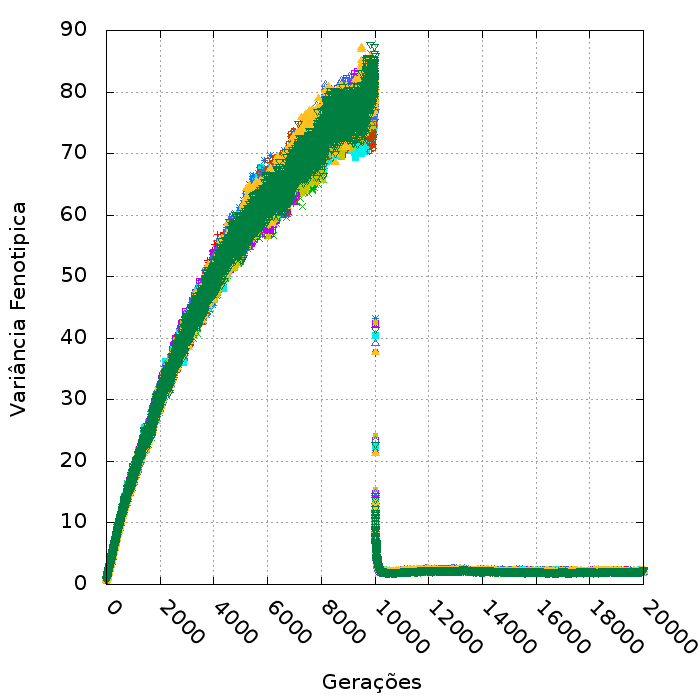
\includegraphics[width=70mm, height=70mm]{figuras/varBurninP.png}}\vspace{11pt}
   \subfloat [Variâncias Genéticas]{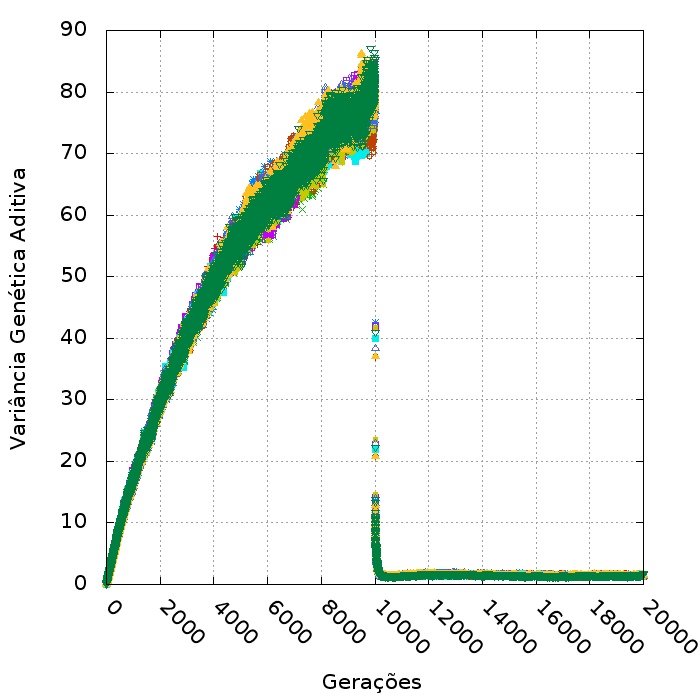
\includegraphics[width=70mm, height=70mm]{figuras/varBurninG.png}}\\ 
   \vspace{-18pt}
   \subfloat [Herdabilidade]{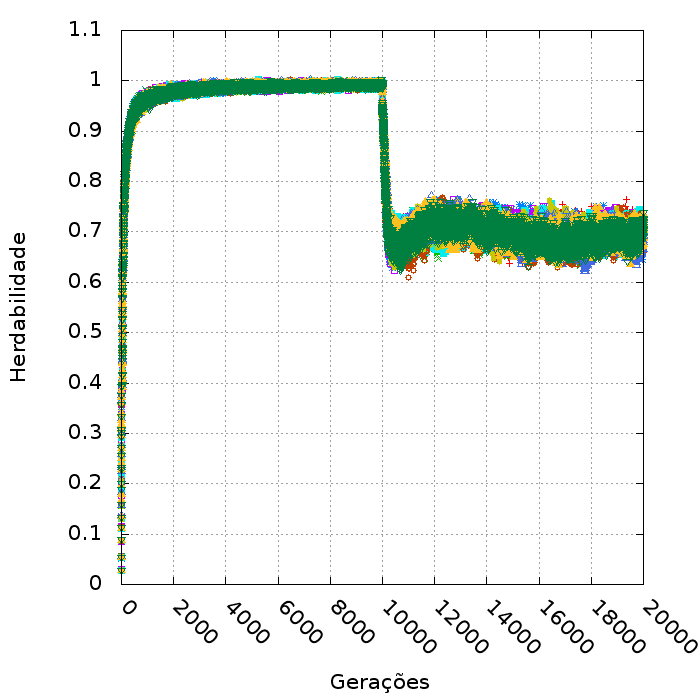
\includegraphics[width=70mm, height=70mm]{figuras/varBurninH.png}}\vspace{11pt} 
   \subfloat [Correlações]{\label{Corr}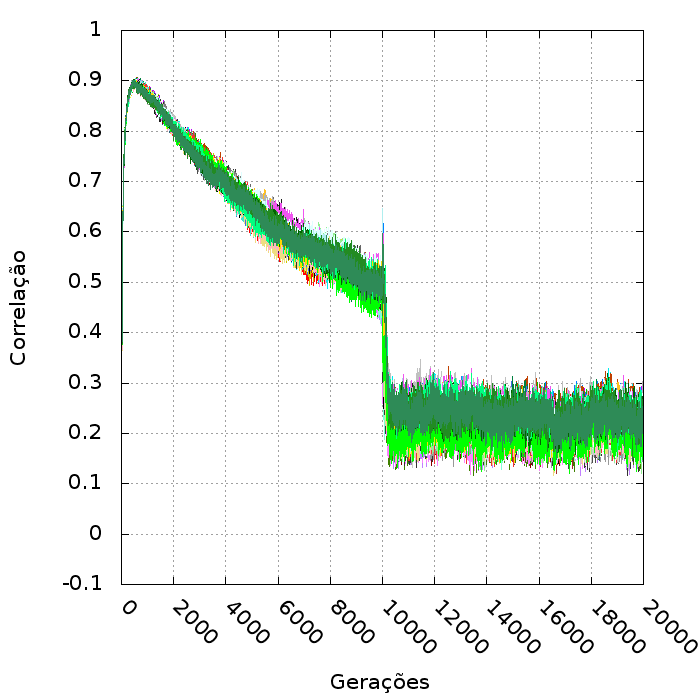
\includegraphics[width=70mm, height=70mm]{figuras/varBurninCorr.png}}\\
   \caption{Evolução de variâncias fenotípicas e genéticas,
   herdabilidades e correlações para uma população passando por 10.000
gerações de deriva, seguidas de 10.000 gerações de seleção
estabilizadora correlacionada ($Ne = 5.000$, $m/p=5$, $\mu/\mu_B=5$).}
   \label{varBurnin}
\end{figure}


\section{Seleção Direcional}

Tomados os cuidados com a inicialização da população, iniciamos o
regime de seleção direcional com intensidade variáveis, como na seção
\ref{cap3:DirecB}. 
Novamente nossa seleção é medida por mudanças no pico adaptativo, com
$\Delta_S$ de $0.01$ até $0.2$. 
Valores de AVG-Ratio e modularidade $L$ para essas corridas podem ser
vistos na figura \ref{MFMStats}. 
Incluímos também, por clareza, as últimas gerações de seleção
estabilizadora, a seleção direcional começa a atuar a partir da geração
20.000. 

Nessa condições o sistema se modulariza rapidamente a partir de uma dada
intensidade de seleção.
Vimos o mesmo efeito na figura \ref{IntSelStats10100}, por exemplo, onde
vemos um aumento tanto da modularidade $L$ quanto do AVG-Ratio,
indicando a presença de modularidade variacional na estrutura de
covariação da população simulada.
Podemos ainda dissecar o efeito da seleção direcional nas correlações
dentro e entre módulos, olhando para a evolução de cada uma
separadamente. 
Na figura \ref{AVGEntreIntra} podemos ver essa separação para diferentes
valores de $\Delta_S$. 
O padrão de aumento das correlações dentro módulos é esperado. 
Além disso, observados uma concomitante diminuição das correlações entre
módulos. 
Novamente, isso é característico de uma estrutura variacional modular,
com duas classes de correlação correspondendo a relação de caracteres
dentro e entre módulos.
Como cada módulo responde a forças seletivas antagônicas a correlação
entre eles tente a diminuir, permitindo que os caracteres dentro de cada
módulo evoluam independentemente dos outros módulos. 
Isso é coerente com simulações em sistemas simples feitas por
\cite{Pavlicev2010} utilizando a equação
de reposta a seleção de \cite{Lande1979} e a existência de rQTLs
\citep{Pavlicev2008a}. 
Neste artigo os autores descrevem como seleção direcional pode favorecer
ativamente a criação de linhas de menor resistência evolutiva
\citep[direções do espaço morfológico ricas em
variação, veja][]{Schluter1996},  alinhadas com a seleção. 
Reorganização de estrutura variacional relacionada a eventos de seleção
prolongada também já foram descritos na literatura \citep{Young2010}. 
Nossos resultados mostram que isso pode acontecer em sistemas
bastante complexos, via seleção indireta nos padrões de
covariação, gerando variação nas direções privilegiadas pela seleção
direcional e aumentando a evolvabilidade das populações. 
Evolvabilidade é definida como a projeção da resposta evolutiva na
direção privilegiada pela seleção natural \citep{Hansen2008}.
Esse valor é controlado por dois fatores: a intensidade da pressão
seletiva, seleção direcional mais intensa provoca mudanças maiores; e
pela quantidade de variação disponível na população na direção da
seleção direcional, caso a população não possua variação herdável na
direção da seleção, não existe resposta evolutiva.
O alinhamento da estrutura de covariação da população com o vetor de
resposta evolutiva basicamente representa o aumento de variação
fenotípica da população na direção da seleção.
Dessa forma, esse tipo de plasticidade na estrutura de covariação pode
ser muito vantajosa, permitindo com que populações sofrendo seleção
direcional aumentem sua variabilidade na direção da seleção, aumentando
sua resposta adaptativa.

\section{Seleção direcional ``corredor''}

Seleção direcional parece então ser fundamental para o surgimento de
módulos variacionais nas nossas simulações. 
Porém, a situação onde todos os caracteres de um complexo morfológico estão
sobre seleção simultânea divergente não parece ser uma regra na
natureza, ou pelo menos é difícil acreditar que todas as instâncias de
modularidade variacional sejam devido a eventos de seleção direcional
divergente em todos os caracteres dos módulos envolvidos simultaneamente. 
Seria a seleção natural sobre apenas um conjuntos de caracteres capaz de
gerar modularidade do mesmo tipo?
Para responder essa pergunta nós começamos com a mesma população
inicial, mas agora apenas um dos módulos era sujeito a seleção
direcional, com o outro conjunto de caracteres mantido constante pela
seleção estabilizadora. 
Novamente a matriz de seleção da superfície adaptativa era não diagonal,
impondo seleção estabilizadora correlacionada na população.
Esse cenário evolutivo é conhecido como evolução ``corredor'', pois uma
parte dos caracteres se altera por ação da seleção direcional (ao
longo do corredor) enquanto o outro conjunto está restrito por ação de
seleção estabilizadora (entre as paredes do corredor). 

Na figura \ref{CoAVG} vemos a evolução das correlações dentro e entre
módulos para esse cenário evolutivo. 
Primeiro destacamos que novamente as correlações entre módulo decaem, de
forma semelhante ao caso de seleção direcional divergente nos dois
módulos. 
O módulo sobre seleção direcional também se comporta de forma semelhante
ao caso anterior, com correlações aumentando ao longo da simulação. 
Porém, nessas simulações são geradas 3 classes de correlação. 
As correlações dentro do módulo sofrendo apenas seleção estabilizadora
também aumentam, ainda que de forma menos acentuada que as do módulo que
sofre seleção direcional. 
Em alguns casos as correlações dentro do módulo com seleção
estabilizadora chegam ao mesmo nível médio que o módulo sofrendo seleção
direcional, como no painel \ref{CoAVG:Igual}. 
À medida que a seleção direcional aumenta, a distinção entre os dois
módulos se torna mais acentuada. 
Esses resultados apontam para um mecanismo plausível de formação de
módulos variacionais em populações naturais. 
Como a seleção em um grupo de caracteres é suficiente para gerar
modularidade na estrutura de covariação completa na população, incluindo
caracteres não diretamente envolvidos na seleção direcional, eventos
subsequentes de seleção direcional em grupos distintos de caracteres
morfológicos podem gerar o padrão intrincado de módulos que observamos na
natureza, sem para isso ser necessária a atuação de seleção direcional
divergente simultânea sobre os módulos. 


\begin{figure}[htbp]
   \centering
   \subfloat [$\Delta_S = 0.01$]{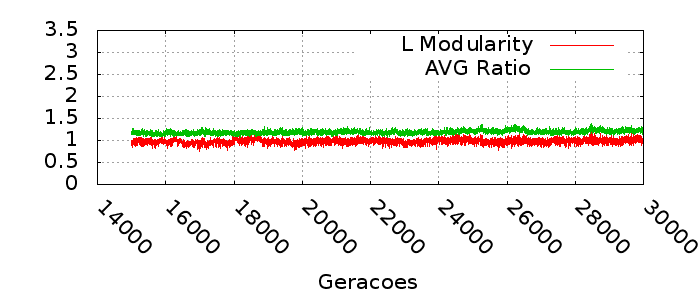
\includegraphics[width=70mm, height=30mm]{figuras/MFMStats10.png}}\vspace{11pt}
   \subfloat [$\Delta_S = 0.03$]{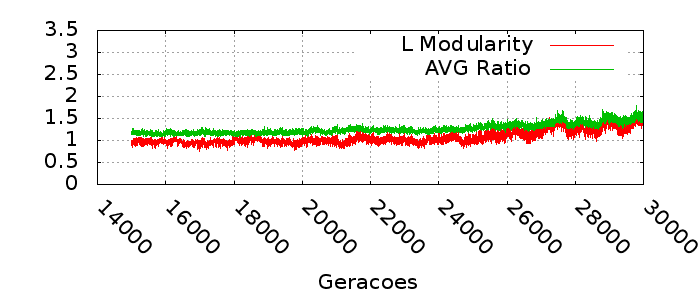
\includegraphics[width=70mm, height=30mm]{figuras/MFMStats30.png}}\\ 
   \vspace{-18pt}
   \subfloat [$\Delta_S = 0.05$]{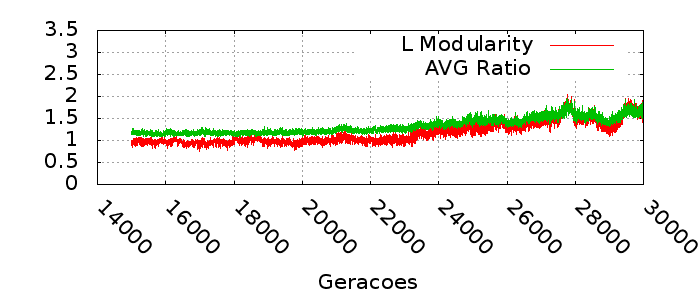
\includegraphics[width=70mm, height=30mm]{figuras/MFMStats50.png}}\vspace{11pt} 
   \subfloat [$\Delta_S = 0.07$]{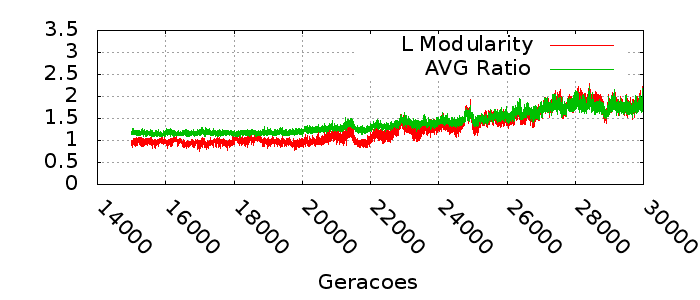
\includegraphics[width=70mm, height=30mm]{figuras/MFMStats70.png}}\\
   \vspace{-18pt}
   \subfloat [$\Delta_S = 0.09$]{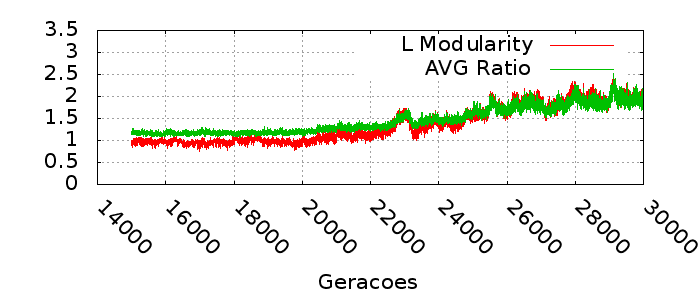
\includegraphics[width=70mm, height=30mm]{figuras/MFMStats90.png}}\vspace{11pt}
   \subfloat [$\Delta_S = 0.11$]{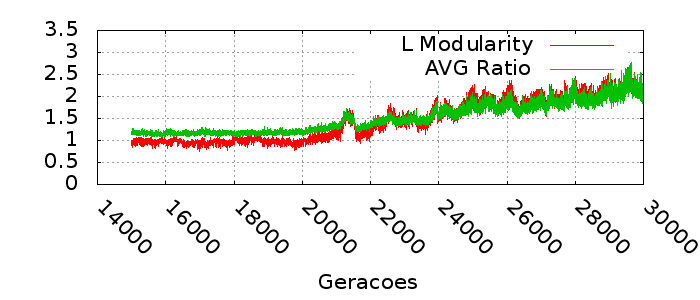
\includegraphics[width=70mm, height=30mm]{figuras/MFMStats110.png}}\\
   \vspace{-18pt}
   \subfloat [$\Delta_S = 0.13$]{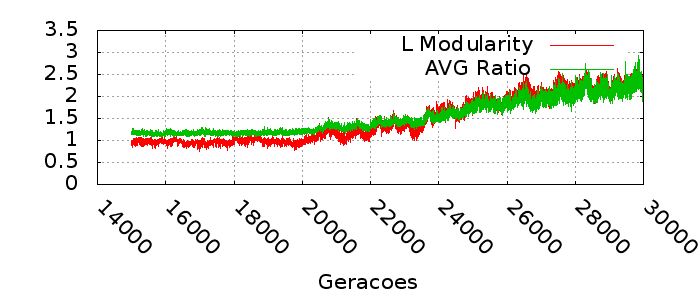
\includegraphics[width=70mm, height=30mm]{figuras/MFMStats130.png}}\vspace{11pt}
   \subfloat [$\Delta_S = 0.15$]{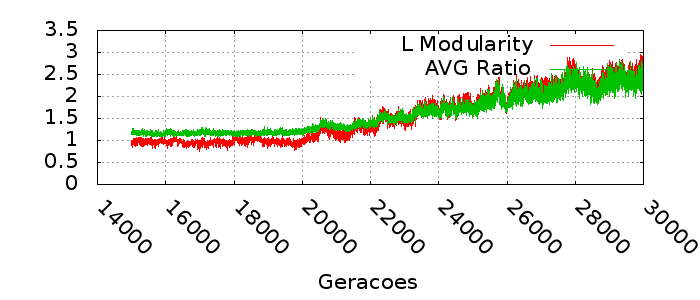
\includegraphics[width=70mm, height=30mm]{figuras/MFMStats150.png}}\\
   \vspace{-18pt}
   \subfloat [$\Delta_S = 0.17$]{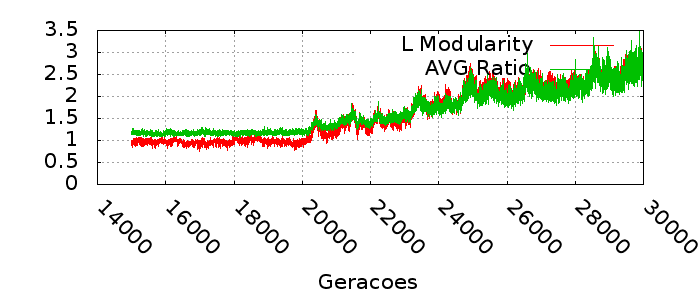
\includegraphics[width=70mm, height=30mm]{figuras/MFMStats170.png}}\vspace{11pt}
   \subfloat [$\Delta_S = 0.19$]{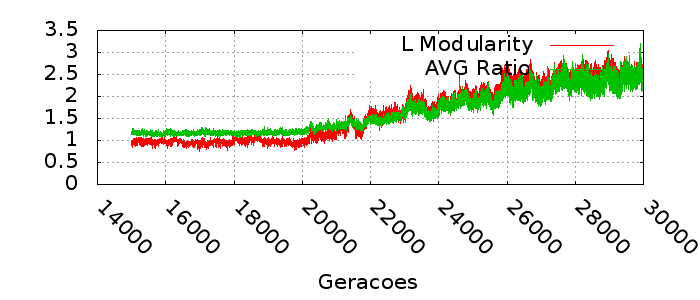
\includegraphics[width=70mm, height=30mm]{figuras/MFMStats190.png}}\\
   \caption{ AVG-Ratio e modularidade $L$ para corridas com
      $\mu/\mu_B = 5$, $Ne = 5.000$, $m/p=5$, sofrendo seleção
      estabilizadora correlacionada com 2 módulos e seleção direcional com
   diferentes valores de $\Delta_S$.}
   \label{MFMStats}
\end{figure}

\begin{figure}[htbp]
   \centering
   \subfloat [$\Delta_S = 0.01$]{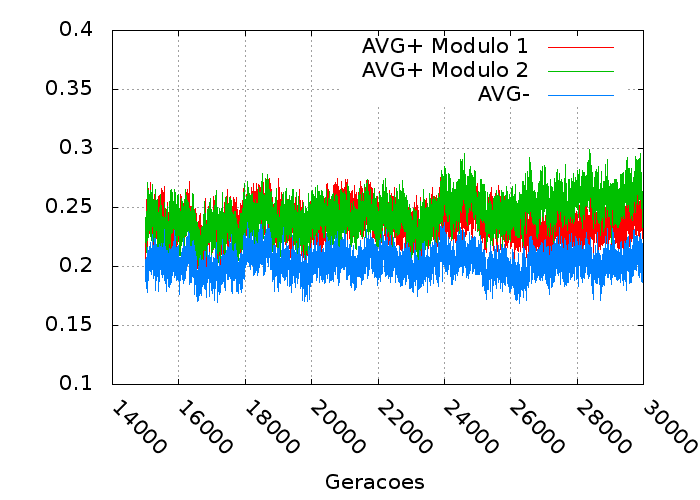
\includegraphics[width=70mm, height=50mm]{figuras/AVGPlusMinus10.png}}\vspace{11pt}
   \subfloat [$\Delta_S = 0.03$]{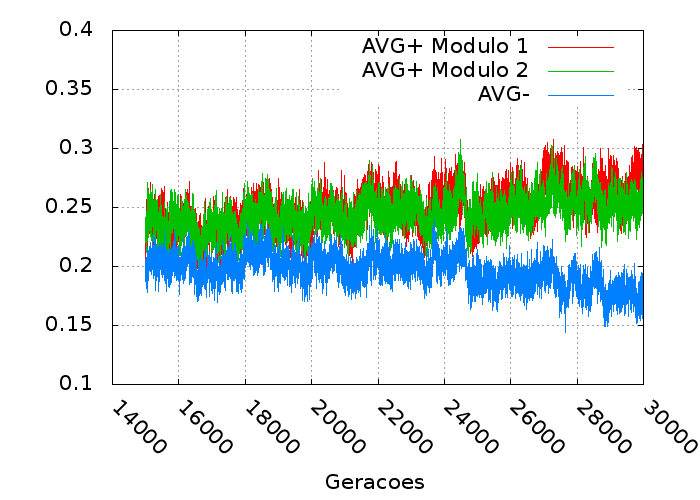
\includegraphics[width=70mm, height=50mm]{figuras/AVGPlusMinus30.png}}\\ 
   \vspace{-18pt}
   \subfloat [$\Delta_S = 0.90$]{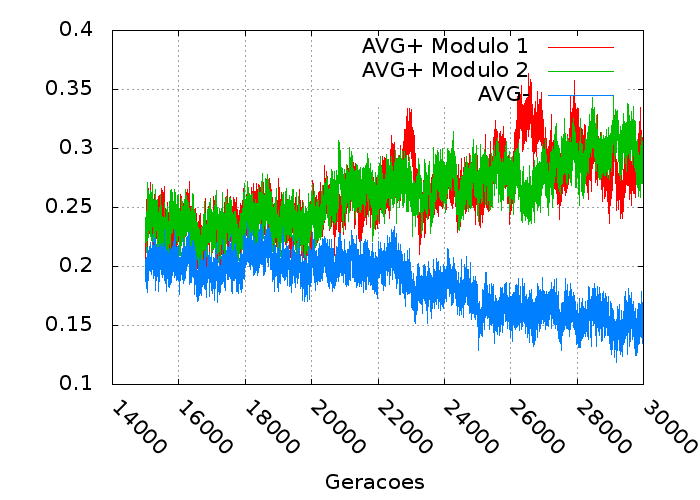
\includegraphics[width=70mm, height=50mm]{figuras/AVGPlusMinus90.png}}\vspace{11pt}
   \subfloat [$\Delta_S = 0.11$]{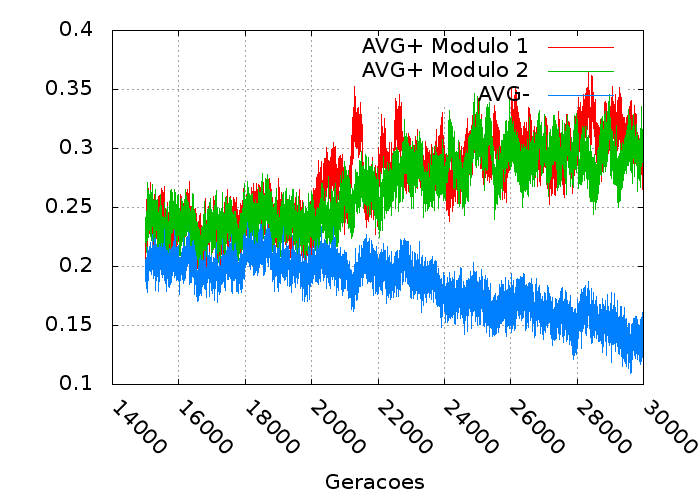
\includegraphics[width=70mm, height=50mm]{figuras/AVGPlusMinus110.png}}\\
   \vspace{-18pt}
   \subfloat [$\Delta_S = 0.18$]{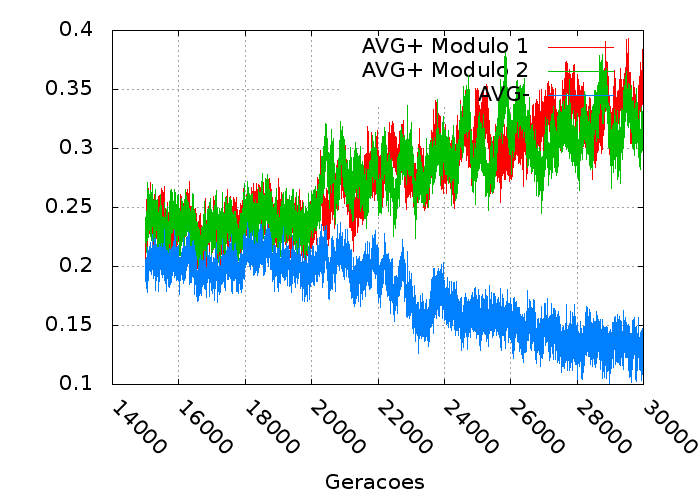
\includegraphics[width=70mm, height=50mm]{figuras/AVGPlusMinus180.png}}\vspace{11pt}
   \subfloat [$\Delta_S = 0.20$]{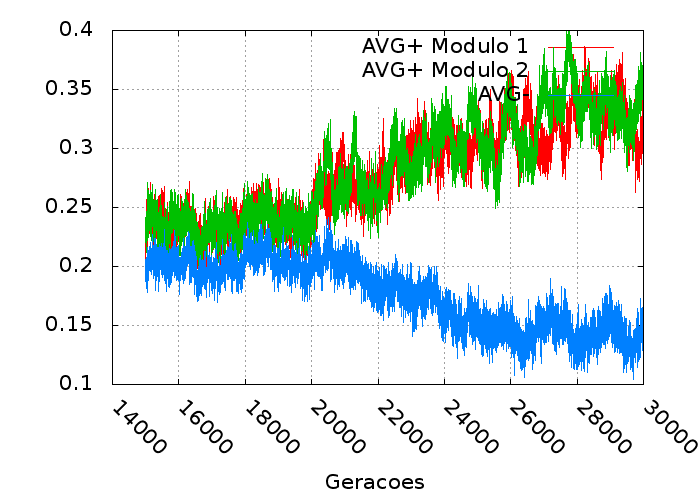
\includegraphics[width=70mm, height=50mm]{figuras/AVGPlusMinus200.png}}\\
   \caption{ Evolução da média das correlações dentro de cada módulo
      e entre módulos de uma população sofrendo seleção estabilizadora
      correlacionada com 2 módulos e seleção direcional com diferentes
   valores de $\Delta_S$. $\mu/\mu_B = 5$, $Ne = 5.000$, $m/p=5$}
   \label{AVGEntreIntra}
\end{figure}

\begin{figure}[htbp]
   \centering
   \subfloat [$\Delta_S = 0.01$]{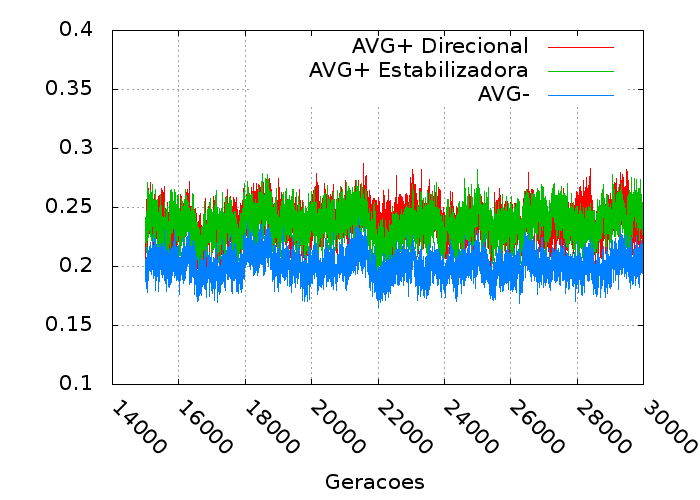
\includegraphics[width=70mm, height=50mm]{figuras/CoAVGPM10.png}}\vspace{11pt}
   \subfloat [$\Delta_S = 0.03$]{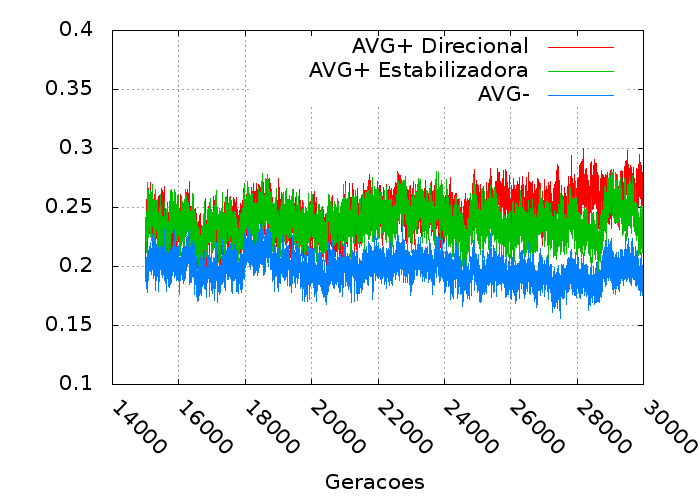
\includegraphics[width=70mm, height=50mm]{figuras/CoAVGPM30.png}}\\ 
   \vspace{-18pt}
   \subfloat [$\Delta_S = 0.90$]{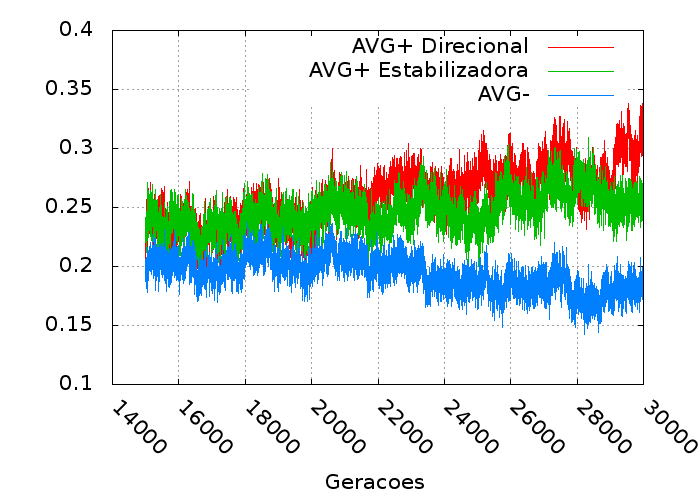
\includegraphics[width=70mm, height=50mm]{figuras/CoAVGPM90.png}}\vspace{11pt}
   \subfloat [$\Delta_S = 0.11$]{\label{CoAVG:Igual}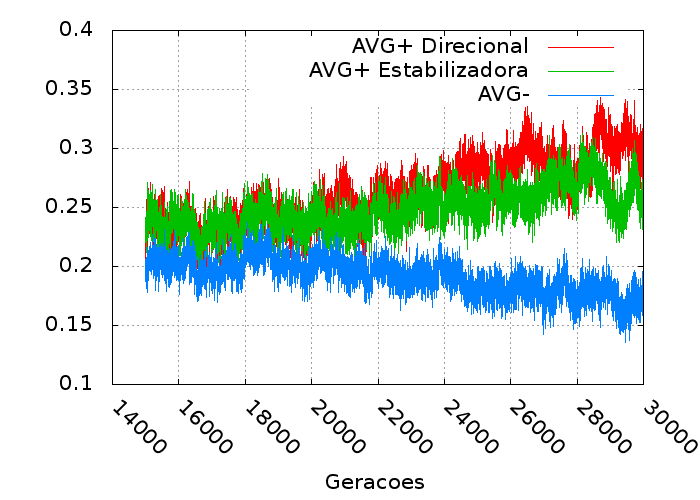
\includegraphics[width=70mm, height=50mm]{figuras/CoAVGPM110.png}}\\
   \vspace{-18pt}
   \subfloat [$\Delta_S = 0.18$]{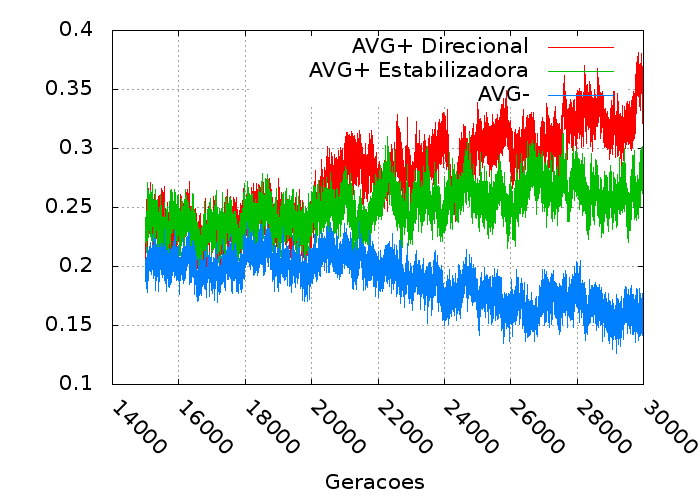
\includegraphics[width=70mm, height=50mm]{figuras/CoAVGPM180.png}}\vspace{11pt}
   \subfloat [$\Delta_S = 0.20$]{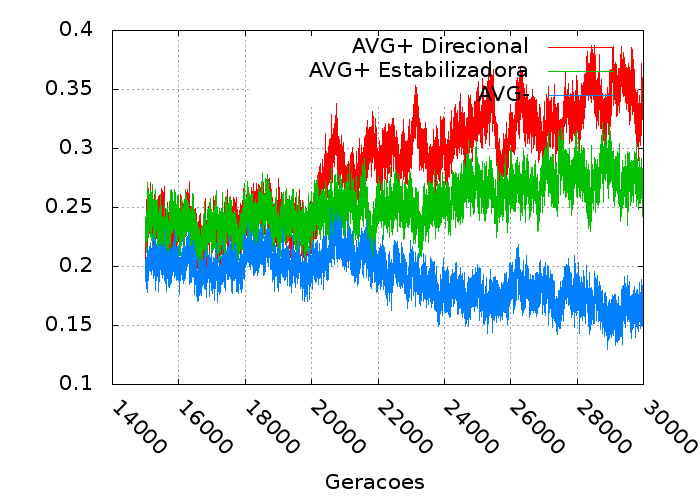
\includegraphics[width=70mm, height=50mm]{figuras/CoAVGPM200.png}}\\
   \caption{ Evolução da média das correlações dentro de cada módulo
      e entre módulos de uma população sofrendo seleção estabilizadora
      correlacionada com 2 módulos e seleção direcional em apenas um dos
   módulos, com diferentes valores de $\Delta_S$. $\mu/\mu_B = 5$, $Ne = 5.000$, $m/p=5$}
   \label{CoAVG}
\end{figure}

